\newpage
\section[Einführung in die Tensorprodukte]{Tensorprodukt}
Das Tensorprodukt verknüpft auf charakteristische Weise zwei Vektorräume miteinander. Die Definitionen mögen sehr trocken wirken, also wäre meine Empfehlung sich zuerst die Beispiele anzugucken und dann die Theorie anpacken.
\subsection{Mathematisches Tensorprodukt}
\begin{Def}{Tensorprodukt}
    Zunächst erweitern wir den Begriff der Billinearform. Statt
    $$\alpha: V\times W \rightarrow \mathbb{K}$$
    gilt nun:
    $$\alpha: V\times W \rightarrow X$$
    wobei $X$ ein Vektorraum ist. \\ \\
    Das \red{Tensorprodukt} kann man sich einfach als eine neue Verknüpfung zwischen Vektorräumen vorstellen. Sie ist definiert über die universelle Eigenschaft:
    \begin{center}
    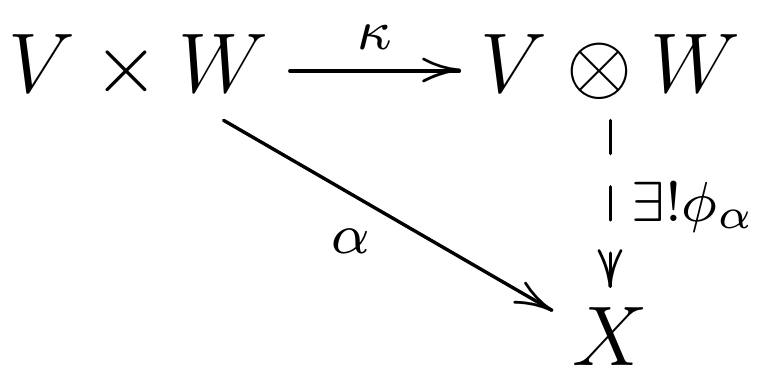
\includegraphics[width=0.3\textwidth]{Dateien/Tensor1.png}
\end{center}
wobei $V\otimes W$ der Tensorproduktraum ist. Diese Definition hat folgende Vorteile: \\
\begin{enumerate}
    \item Jeder bilinearen Abbildung $\alpha$ kann genau eine Lineare Abbildung $\Phi_\alpha$ zugeordent werden.
    \item Der Tensorproduktraum ist bis auf Isomorphie eindeutig. Seien nämlich zwei Räume $V\otimes W$ und $V\Tilde{\otimes}W$ gegeben, dann gilt für $X=V\Tilde{\otimes}W$:
\begin{center}
    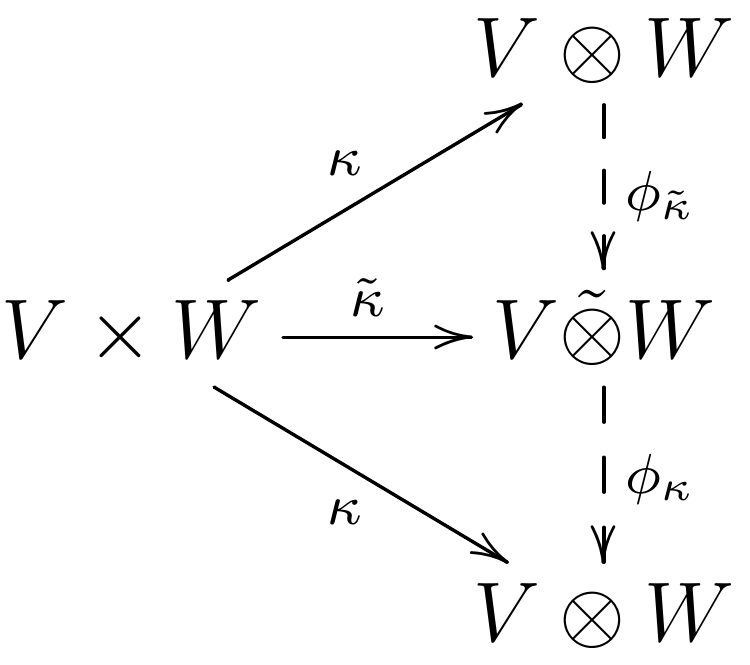
\includegraphics[width=0.28\textwidth]{Dateien/Tensor2.png}
\end{center}
und damit $$\Phi_\kappa \circ \Phi_{\Tilde{\kappa}}=Id_{V\Tilde{\otimes}W} \quad \Phi_{\Tilde{\kappa}} \circ \Phi_\kappa  =Id_{V\otimes W}$$
Die Abbildungen $\Phi_\kappa$, $\Phi_{\Tilde{\kappa}}$ sind also gegenseitige Umkehrabbildungen und damit Bijektiv!
\item Das Tensorprodukt existiert! Seien dazu $V$ und $W$ Vektorräume mit den Basen $b_i$ und $b_j$ und:
$$\mathcal{V}(V\times W)=\{ T: V\times W \rightarrow \mathbb{K}, T\neq 0 \}$$
Eine Basis von $\mathcal{V}(V\times W)$ ist dann gegeben durch:
$$\delta_{(b_i, b_j)}(V,W)=\begin{cases}
    1 & \mbox{ wenn $v=b_i$ und $w=b_j$} \\
    0 & \mbox{ sonst}
\end{cases}$$
Wir schreiben nun:
$$\alpha(V,W) = \alpha(\sum_i \lambda_ib^i, \sum_j \mu_jb^{,j})=\sum_{i,j} T_{ij}\alpha(b^i, b^{,j})$$
$$\kappa(V, W)= \kappa(\sum_i \lambda_ib^i, \sum_j \mu_jb^{,j})=\sum_{i,j} T_{ij}\delta_{(b^i, b^{,j})}$$
$$\Phi_\alpha(T)=\Phi_\alpha(\sum_{i,j} T_{ij}\delta_{(b^i, b^{,j})})=\sum_{i,j}T_{ij}\alpha(b^i, b^{,j})$$
Bildlich passiert also folgendes:
\begin{center}
    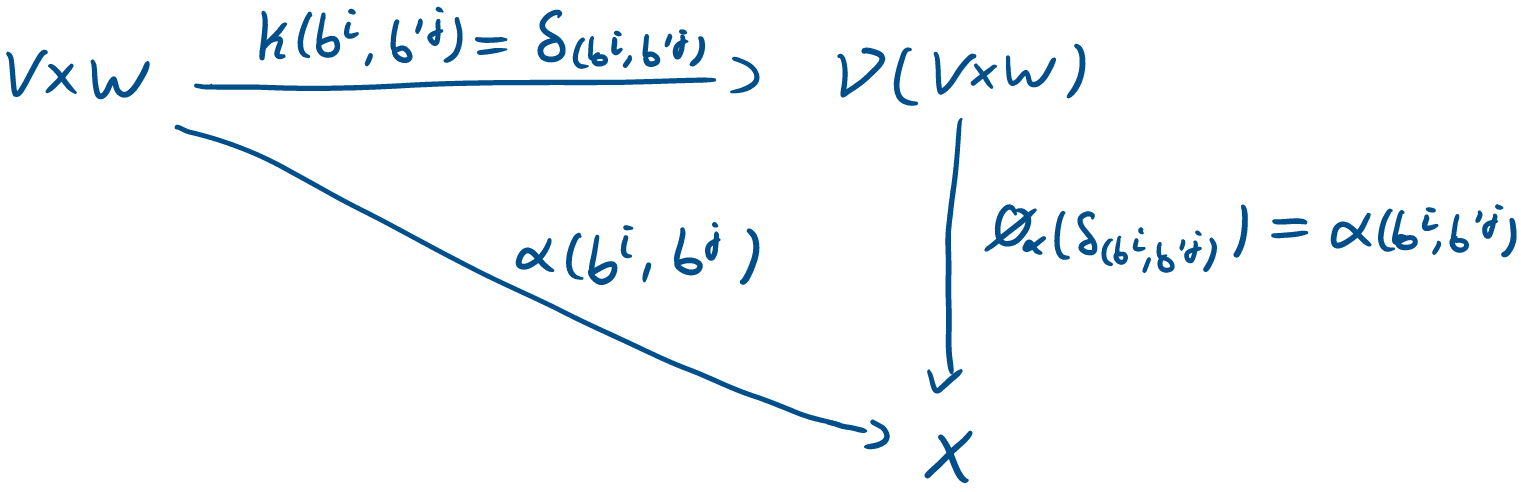
\includegraphics[width=0.7\textwidth]{Dateien/Tensor3.png}
\end{center}
Diese Definitionen erfüllen alle benötigten Eigenschaften. Allegemin schreibt man:
$$\kappa(b^i, b^{,j})=b^i\otimes b^{,j}$$
\end{enumerate}
\end{Def}

\begin{Satz}{Regeln}{Eigenschaften des Tensorprodukts}
\begin{enumerate}
    \item Für endlichdimensionale Vektorräume gilt
    $$dim_{\mathbb{K}}V\otimes W = dim_{\mathbb{K}} V \cdot dim_{\mathbb{K}} W$$
    \item Sind $V,W$ Hilberträume, lässt sich das Skalarprodukt erweitern:
    $$\braket{v\otimes w, v'\otimes w'}=\braket{v,v'}\cdot \braket{w, w'} \quad \forall v,v'\in V\quad w,w'\in W$$
    \item Es sei $$\alpha: V\rightarrow V' \quad \beta:W\rightarrow W' \quad \alpha\otimes\beta. V\otimes W \rightarrow V'\otimes W'$$
    dann gilt:
    $$(\alpha\otimes\beta)(V\otimes W)=\alpha(V)\otimes \beta(W)$$
    \item Das Tensorprodukt ist bilinear:
    $$(\lambda_1\Phi_1+\lambda_2\Phi_2)\otimes \Psi = \lambda_1\Phi_1 \otimes \Psi + \lambda_2\Phi_2 \otimes \Psi$$
    $$\Phi\otimes (\lambda_1\Psi_1+ \lambda_2\Psi_2) = \lambda_1\Phi \otimes \Psi_1 + \lambda_2\Phi \otimes \Psi_2$$
    \item Elemente der Form
    $$V\otimes W=\kappa(V,W)$$
    heißen Tensorprodukte oder reine Tensoren. Es gibt aber auch Elemente, die die Eigenschaft nicht erfüllen, wie zum Beispiel:
    $$b^1\otimes b^{,1}+b^2\otimes b^{,2}$$
\end{enumerate}
\end{Satz}
\begin{Def}{Transformation von Tensoren}
    Wir betrachten die Vektorräume $V,V'$ mit Basen $e_i$ und $e_i'$ sowie $W, W'$ mit Basen $f_i, f_i'$. Für lineare Abbildungen $\Phi$ und $\Psi$ gilt:
    $$\Phi(e_i)=\sum_k a^k _i e_k' \quad \Psi(f_i)=\sum_l a^k _e e_k'$$
    und daraus folgt:
    $$(\Phi \otimes \Psi)(x^{ij}e_i\otimes f_j) =x^{ij}a^k_i b^l_j e_k'\otimes f_l'$$
    obere Indizes werden kovariant transformiert
    $$x^{ij}\mapsto x^{ij}a^k_ib^l_j$$
\end{Def}

\begin{Def}{$k$-fache äußere Produkt}
Das \red{$k$-fache äußere Produkt} eines $\mathbb{K}$-Vektorraums $V$ ist ein Vektorraum $\Lambda^k(V)$, zusammen mit einer $k$-multilinearen alternierenden Abbildung $\wedge: V\times \dots \times V \rightarrow \Lambda^kV$, so dass es für jede $k$-lineare alternierende Abbildung $\alpha: V^k\rightarrow W$ genau eine lineare Abbildung $\Phi_\alpha:\Lambda^kV\rightarrow W$ gibt, so dass das Diagramm.
\begin{center}
    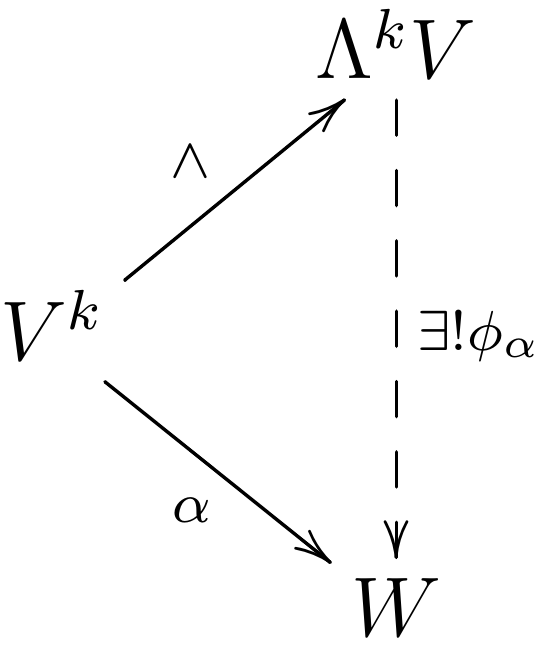
\includegraphics[width=0.28\textwidth]{Dateien/Tensor4.png}
\end{center}
kommutiert.    
\end{Def}
Besonders die letzte Definition ist sehr wichtig für spätere Kapitel.
\newpage
\begin{Beispiel}{Einfaches Tensorprodukt von \href{https://www.math3ma.com/blog/the-tensor-product-demystified}{math3ma.com}}
    Seien $V\subseteq \R^3$ und $W\subseteq \R^2$ und wir suchen uns zwei Vektoren aus.
    $$\vec{v}=\begin{pmatrix}
        1 \\
        2 \\
        3 \\
    \end{pmatrix} \qquad \vec{w}=\begin{pmatrix}
        4 \\
        5 \\
    \end{pmatrix}$$
    Wie können wir aus diesen zwei Vektoren einen neuen erstellen? \\
    \begin{enumerate}
        \item mit der Direkten Summe
        \blue{$$\begin{pmatrix}
        1 \\
        2 \\
        3 \\
    \end{pmatrix} \oplus\begin{pmatrix}
        4 \\
        5 \\
    \end{pmatrix} = \begin{pmatrix}
        1 \\
        2\\
        3\\
        4\\
        5\\
    \end{pmatrix}$$
    $$dim(\R^3\oplus \R^2)=dim(\R^3)+dim(\R^2)=5$$}
    \item mit dem Tensorprodukt
    \blue{$$\begin{pmatrix}
        1 \\
        2 \\
        3 \\
    \end{pmatrix} \otimes\begin{pmatrix}
        4 \\
        5 \\
    \end{pmatrix} = \begin{pmatrix}
        1\cdot 4 \\
        1\cdot 5\\
        2\cdot 4\\
        2\cdot 5\\
        3\cdot 4\\
        3\cdot 5
    \end{pmatrix}=\begin{pmatrix}
        4 \\
        5\\
        8\\
        10\\
        12\\
        15
    \end{pmatrix}$$
    $$dim(\R^3\otimes \R^2)=dim(\R^3)\cdot dim(\R^2)=6$$}
    \end{enumerate}
    Das Tensorprodukt ist wie eine erwachsene Version der Multiplikation. Die Basisvektoren von unseren Tensorprodukt sind auch Tensorprodukte der Basisvektoren der jeweiligen Vektorräumen
    $$\begin{pmatrix}
        4 \\
        5\\
        8\\
        10\\
        12\\
        15
    \end{pmatrix}= 4(e_1\otimes e_1) + 5(e_1\otimes e_2)+8(e_2\otimes e_1) + 10(e_2\otimes e_2) + 12(e_3\otimes e_1) + 15(e_3\otimes e_2)$$
\end{Beispiel}
Guckt euch gerne noch die Website an, weil math3ma Tensoren super erklärt.
\begin{Beispiel}{Tensorprodukte in der Quantenmechanik}
    Der Spinzustand $\ket{\chi}$ lebt in Spinraum $H_s$ und der Ortszustand $\ket{\psi}$ im Ortsraum $H_r$. Der Gesamtzustand lebt im Tensorproduktraum
    $$\ket{\chi}\otimes\ket{\psi} \in H_r\otimes H_s$$
    Auch Vielteilchenzustände sind Tensorprodukte von Einteilchenzuständen.
\end{Beispiel}
\begin{Beispiel}{Nützliche Tensorwerkzeuge aus den Präsenzaufgaben}
\begin{enumerate}
    \item Jedes Element von $V\otimes W$ lässt sich schreiben als
    \blue{$$v_1\otimes w_1 + v_2\otimes w_2 \quad \mbox{mit $v_1,v_2\in V$ und $w_1,w_2\in W$}$$}
    \item Ein \red{reiner Tensor} hat immer die Form
    \blue{$$a\otimes b \quad \mbox{$a\in V$ und $v\in W$}$$}
    \item Wie finden wir ein Element von $\R^3 \otimes \R^2$, dass nicht als ein reiner Tensor dargestellt werden kann?\\
    \blue{Am besten wir stellen uns eine Matrix auf und versuchen dann so eine zu finden, deren Rang mindestens 2 ist
    $$
      ^{e_1}_{e_2}\begin{cases}
          \overbrace{\begin{pmatrix}
     1 & 0 & 0\\
     0 & 1 & 0
  \end{pmatrix}}^{e_1 \quad e_2 \quad e_3}
      \end{cases}$$
      Und tatsächlich haben wir hier schon so eine Matrix gefunden und unser Tensor ist $$e_1\otimes e_1+e_2\otimes e_2$$}
      \item Zeige, dass $x\in V\otimes V$ ungleich Null ist:
      \blue{$$x=\begin{pmatrix}
          3 \\ 0
      \end{pmatrix}\otimes \begin{pmatrix}
          2 \\ 3
      \end{pmatrix}+\begin{pmatrix}
          0 \\ 9
      \end{pmatrix}\otimes \begin{pmatrix}
          1 \\ 0
      \end{pmatrix}=\begin{pmatrix}
          6 \\ 9 \\ 0 \\ 0
      \end{pmatrix}+ \begin{pmatrix}
          0 \\ 0 \\ 9 \\ 0
      \end{pmatrix}=\begin{pmatrix}
          6 \\ 9 \\ 9 \\ 0
      \end{pmatrix}\neq 0$$}
      \item Sei $y\in \Lambda^2 V$. Zeige, dass $y=0$:
      
      \blue{$$y=\begin{pmatrix}
          3 \\ 0
      \end{pmatrix}\wedge \begin{pmatrix}
          2 \\ 3
      \end{pmatrix}+\begin{pmatrix}
          0 \\ 9
      \end{pmatrix}\wedge \begin{pmatrix}
          1 \\ 0
      \end{pmatrix}$$
      Hier ist vorerst die Definition des} \red{2D-Dachproduktes} \blue{wichtig}. 
      \red{$$a\wedge b = \det \begin{pmatrix}
          a_1 & a_2 \\
          b_1 & b_2
      \end{pmatrix}= a_1b_2-a_2b_1$$}
      \blue{$$y=9-9=0$$}
\end{enumerate}
\end{Beispiel}